\documentclass[11pt,a4paper]{article}

% ---------- Paquetes ----------
\usepackage[utf8]{inputenc}
\usepackage[T1]{fontenc}
\usepackage{geometry}
\geometry{margin=2.3cm}
\usepackage{tikz}
\usetikzlibrary{shapes.geometric, shapes.symbols, arrows.meta, positioning, calc}
\usepackage{booktabs}
\usepackage{longtable}
\usepackage{array}
\usepackage{enumitem}
\usepackage{hyperref}
\usepackage{xcolor}
\usepackage{titlesec}
\usepackage{fancyhdr}
\usepackage{algorithm}
\usepackage{algpseudocode}
\usepackage{parskip}

\hypersetup{
    colorlinks=true,
    linkcolor=blue!50!black,
    urlcolor=blue!50!black,
    citecolor=blue!50!black,
    pdftitle={Especificacion del flujo de arranque y ejecucion - Consola FPGA},
    pdfauthor={Proyecto PBL - Digital 1}
}

\pagestyle{fancy}
\fancyhf{}
\fancyhead[L]{Consola de Videojuegos FPGA -- Especificaci\'on de Flujo}
\fancyhead[R]{\thepage}
\renewcommand{\headrulewidth}{0.3pt}

\titleformat{\section}{\normalfont\Large\bfseries}{\thesection}{1em}{}
\titleformat{\subsection}{\normalfont\large\bfseries}{\thesubsection}{1em}{}

% ---------- Estilos TikZ para el flowchart ----------
\tikzstyle{startstop} = [rectangle, rounded corners, minimum width=3.2cm, minimum height=0.9cm,
    text centered, text width=3cm, draw=black, fill=violet!12, font=\small]
\tikzstyle{process} = [rectangle, minimum width=3.4cm, minimum height=0.9cm,
    text centered, text width=3.2cm, draw=black, fill=blue!6, font=\small]
\tikzstyle{io} = [trapezium, trapezium left angle=70, trapezium right angle=110,
    minimum width=3.2cm, minimum height=0.9cm, text width=2.7cm,
    text centered, draw=black, fill=orange!10, font=\small]
\tikzstyle{decision} = [diamond, aspect=2.4, minimum width=3.6cm, minimum height=1.1cm,
    text centered, text width=2.6cm, draw=black, fill=yellow!15, font=\scriptsize, inner sep=1pt]
\tikzstyle{check} = [ellipse, minimum width=3.4cm, minimum height=1cm,
    text centered, text width=2.7cm, draw=black, fill=green!10, font=\scriptsize]
\tikzstyle{arrow} = [thick, -{Stealth[length=2.5mm]}]
\tikzstyle{lbl} = [font=\scriptsize, fill=white, inner sep=1pt]

\newcommand{\grp}[1]{\textcolor{blue!50!black}{\textbf{[#1]}}}

\begin{document}

% =============================================================
\begin{titlepage}
\centering
\vspace*{2cm}
{\LARGE \bfseries Especificaci\'on del Flujo de Arranque, Gesti\'on de Perif\'ericos y Ejecuci\'on\par}
\vspace{0.5cm}
{\Large Consola de Videojuegos Retro sobre FPGA\par}
\vspace{1.5cm}
{\large Proyecto PBL --- Curso Dise\~no Digital 1\par}
\vspace{0.3cm}
{\large Checkpoint 1: Flowchart y especificaci\'on de registros CSR\par}
\vfill
{\large 24 de septiembre de 2026\par}
\end{titlepage}

\tableofcontents
\newpage

% =============================================================
\section{Introducci\'on y arquitectura de referencia}

Este documento especifica formalmente el flujo de control del firmware que gobierna
la consola de videojuegos retro implementada sobre el SoC descrito en
\texttt{diagrama\_soc\_digital1\_v3.svg}. El procesador (\texttt{femtorv32\_quark}, RV32I)
se trata como caja negra; toda la l\'ogica aqu\'i descrita corresponde al firmware en C
que controla, a trav\'es de registros mapeados en memoria (CSR), los perif\'ericos
dise\~nados por cada equipo del curso.

\subsection{Convenci\'on de grupos}
Cada nodo del flujo indica, entre par\'entesis, el o los grupos responsables del
m\'odulo RTL y/o firmware involucrado. Esta trazabilidad es la que permite que, aunque
la plataforma sea \'unica y compartida, cada equipo pueda verificar de forma aislada
la porci\'on del flujo que le corresponde.

\begin{table}[h]
\centering
\small
\begin{tabular}{@{}cll@{}}
\toprule
\textbf{Grupo} & \textbf{M\'odulo RTL / responsabilidad} & \textbf{Rango de memoria} \\
\midrule
A & \texttt{bram.v} --- memoria de arranque / firmware & 0x000000 -- 0x3FFFFF \\
B & \texttt{perip\_uart.v} --- diagn\'ostico serie & 0x400000 -- 0x40FFFF \\
C & \texttt{perip\_spiram.v} --- RAM de trabajo externa & 0x410000 -- 0x41FFFF \\
D & \texttt{perip\_spiflash.v} --- almacenamiento de assets/firmware & 0x420000 -- 0x42FFFF \\
E & \texttt{perip\_ps2kbd.v} --- teclado PS/2 & 0x430000 -- 0x43FFFF \\
F & \texttt{perip\_ps2mouse.v} --- mouse PS/2 & 0x440000 -- 0x44FFFF \\
G & \texttt{perip\_nes.v} --- control tipo NES & 0x450000 -- 0x45FFFF \\
I & \texttt{perip\_i2s.v} --- audio & 0x470000 -- 0x47FFFF \\
J & \texttt{perip\_display.v} --- framebuffer / panel & 0x480000 -- 0x4FFFFF \\
K & \texttt{software\_juegos} --- l\'ogica de juego / firmware de integraci\'on & --- \\
L & LEDs RGB de puerto y pantallas laterales (perif\'erico adicional) & --- \\
\bottomrule
\end{tabular}
\caption{Trazabilidad grupo $\rightarrow$ m\'odulo, seg\'un el mapa de memoria del SoC.}
\end{table}

\noindent\textit{Nota:} el grupo H (I2C / EEPROM de puntajes) no participa del flujo
principal de arranque--men\'u--ejecuci\'on; su interacci\'on se documenta por separado
en los subdiagramas de protocolo I\textsuperscript{2}C (\S\ref{sec:pendientes}).

\subsection{Leyenda de formas}
\begin{center}
\resizebox{\textwidth}{!}{%
\begin{tikzpicture}[node distance=2.6cm]
\node (a) [startstop] {Inicio / Fin};
\node (b) [process, right=of a] {Proceso};
\node (c) [io, right=of b] {Entrada / Salida};
\node (d) [decision, right=of c, xshift=0.3cm] {Decisi\'on};
\node (e) [check, right=of d, xshift=0.3cm] {Verificaci\'on / chequeo};
\end{tikzpicture}}
\end{center}

% =============================================================
\section{Fase 1 --- Arranque y diagn\'ostico}
\label{sec:fase1}

\subsection{Diagrama}
\begin{center}
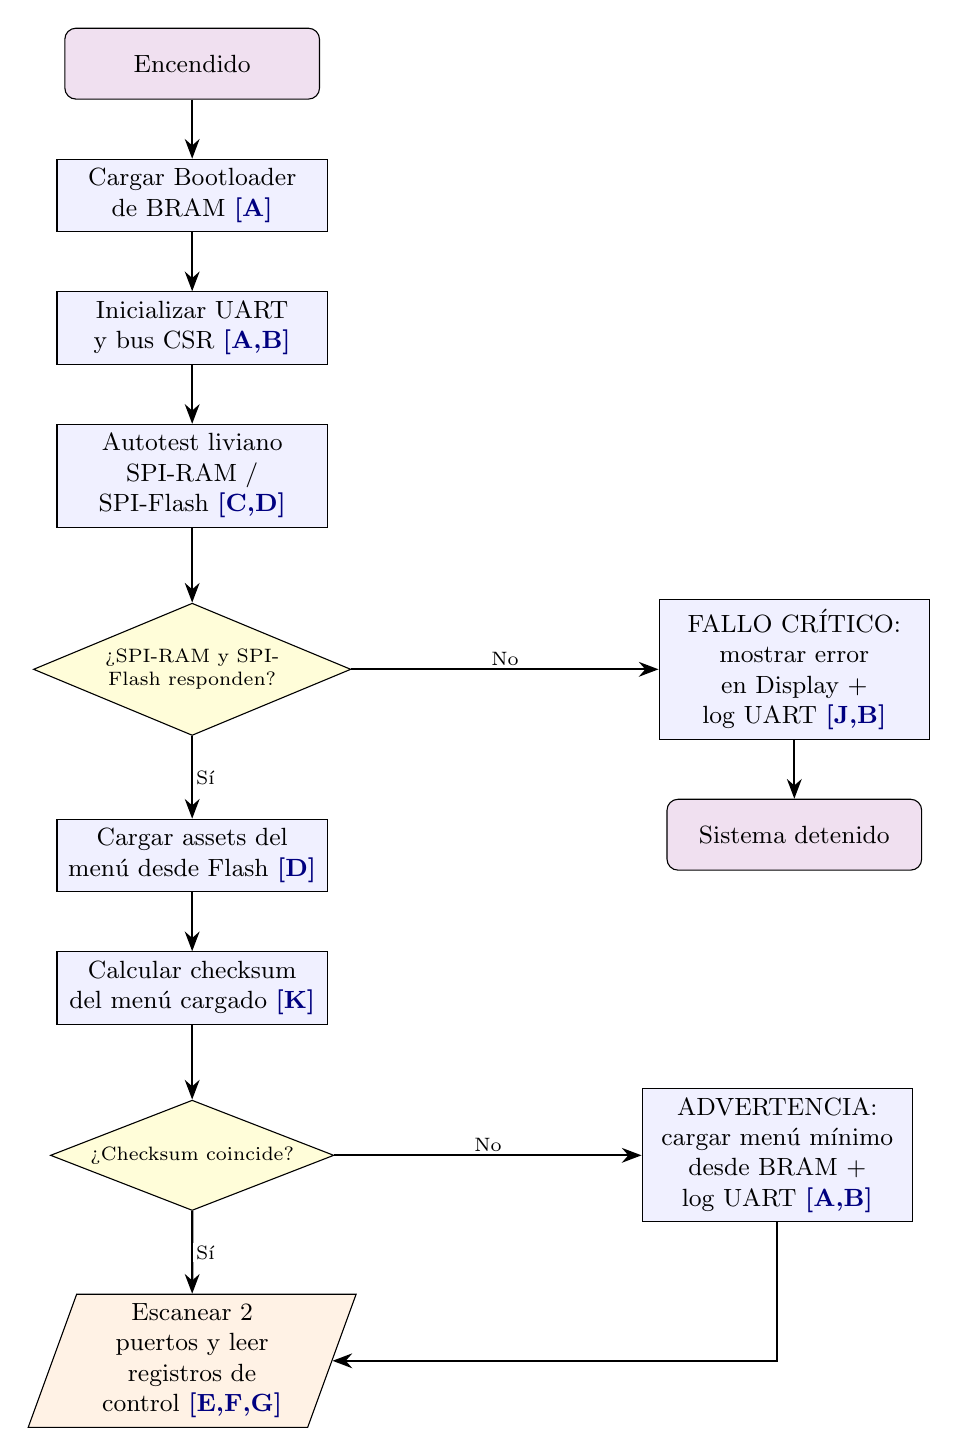
\begin{tikzpicture}[node distance=0.75cm and 2.2cm]
\node (power) [startstop] {Encendido};
\node (boot) [process, below=of power] {Cargar Bootloader de BRAM \grp{A}};
\node (init) [process, below=of boot] {Inicializar UART y bus CSR \grp{A,B}};
\node (self) [process, below=of init] {Autotest liviano SPI-RAM / SPI-Flash \grp{C,D}};
\node (hwok) [decision, below=of self, yshift=-0.2cm] {\textquestiondown SPI-RAM y SPI-Flash responden?};
\node (hardfail) [process, right=of hwok, xshift=1.7cm] {FALLO CR\'ITICO: mostrar error en Display + log UART \grp{J,B}};
\node (stop) [startstop, below=of hardfail] {Sistema detenido};
\node (loadmenu) [process, below=of hwok, yshift=-0.3cm] {Cargar assets del men\'u desde Flash \grp{D}};
\node (chk) [process, below=of loadmenu] {Calcular checksum del men\'u cargado \grp{K}};
\node (chkok) [decision, below=of chk, yshift=-0.2cm] {\textquestiondown Checksum coincide?};
\node (softfail) [process, right=of chkok, xshift=1.7cm] {ADVERTENCIA: cargar men\'u m\'inimo desde BRAM + log UART \grp{A,B}};
\node (scanports) [io, below=of chkok, yshift=-0.3cm] {Escanear 2 puertos y leer registros de control \grp{E,F,G}};

\draw[arrow] (power) -- (boot);
\draw[arrow] (boot) -- (init);
\draw[arrow] (init) -- (self);
\draw[arrow] (self) -- (hwok);
\draw[arrow] (hwok) -- node[lbl,above]{No} (hardfail);
\draw[arrow] (hardfail) -- (stop);
\draw[arrow] (hwok) -- node[lbl,right]{S\'i} (loadmenu);
\draw[arrow] (loadmenu) -- (chk);
\draw[arrow] (chk) -- (chkok);
\draw[arrow] (chkok) -- node[lbl,above]{No} (softfail);
\draw[arrow] (softfail) |- (scanports);
\draw[arrow] (chkok) -- node[lbl,right]{S\'i} (scanports);
\end{tikzpicture}
\end{center}

\subsection{Descripci\'on}
La Fase 1 garantiza que el sistema pueda alcanzar un estado usable incluso ante
fallos parciales de hardware, distinguiendo dos niveles de severidad:

\begin{itemize}[leftmargin=1.4em]
    \item \textbf{Fallo duro} (SPI-RAM o SPI-Flash no responden al patr\'on de prueba):
    detiene el sistema, pero mantiene el reporte de error operativo porque BRAM,
    UART y Display est\'an en rangos de memoria independientes de SPI-RAM/Flash
    (v\'ease Tabla~1), por lo que no dependen del subsistema que fall\'o.
    \item \textbf{Fallo blando} (checksum del men\'u no coincide): el sistema
    no se detiene; degrada a un men\'u de emergencia embebido en BRAM y contin\'ua
    el flujo normal hacia el escaneo de puertos.
\end{itemize}

\begin{algorithm}[H]
\caption{Fase 1 --- Arranque y diagn\'ostico}
\begin{algorithmic}[1]
\State cargar\_bootloader\_bram()
\State inicializar\_uart\_y\_bus\_csr()
\State ok $\gets$ autotest\_liviano(SPIRAM, SPIFLASH)
\If{$\lnot$ ok}
    \State mostrar\_error\_critico(Display, UART)
    \State \textbf{detener sistema}
\Else
    \State cargar\_assets\_menu\_desde\_flash()
    \State chk $\gets$ calcular\_checksum(menu\_cargado)
    \If{chk $\neq$ chk\_esperado}
        \State advertencia\_no\_bloqueante(BRAM, UART)
    \EndIf
    \State escanear\_puertos()  \Comment{contin\'ua en Fase 2}
\EndIf
\end{algorithmic}
\end{algorithm}

% =============================================================
\section{Fase 2 --- Gesti\'on de perif\'ericos}
\label{sec:fase2}

\subsection{Diagrama}
\begin{center}
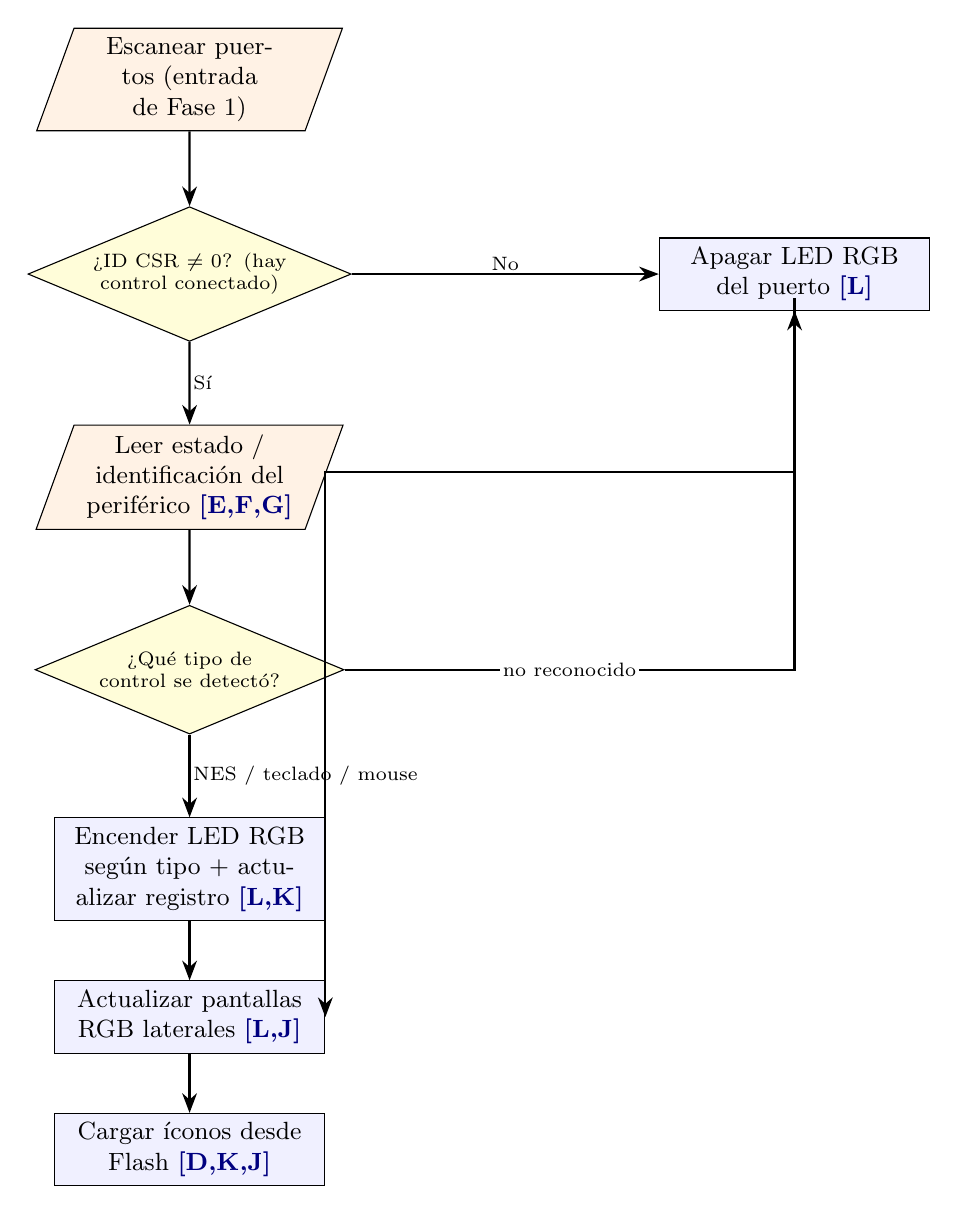
\begin{tikzpicture}[node distance=0.75cm and 2.2cm]
\node (scan) [io] {Escanear puertos (entrada de Fase 1)};
\node (isconn) [decision, below=of scan, yshift=-0.2cm] {\textquestiondown ID CSR $\neq$ 0? (hay control conectado)};
\node (ledoff) [process, right=of isconn, xshift=1.7cm] {Apagar LED RGB del puerto \grp{L}};
\node (readsig) [io, below=of isconn, yshift=-0.3cm] {Leer estado / identificaci\'on del perif\'erico \grp{E,F,G}};
\node (idtype) [decision, below=of readsig, yshift=-0.2cm] {\textquestiondown Qu\'e tipo de control se detect\'o?};
\node (ledon) [process, below=of idtype, yshift=-0.3cm] {Encender LED RGB seg\'un tipo + actualizar registro \grp{L,K}};
\node (ctrlrgb) [process, below=of ledon] {Actualizar pantallas RGB laterales \grp{L,J}};
\node (loadicons) [process, below=of ctrlrgb] {Cargar \'iconos desde Flash \grp{D,K,J}};

\draw[arrow] (scan) -- (isconn);
\draw[arrow] (isconn) -- node[lbl,above]{No} (ledoff);
\draw[arrow] (isconn) -- node[lbl,right]{S\'i} (readsig);
\draw[arrow] (readsig) -- (idtype);
\draw[arrow] (idtype) -- node[lbl,right]{NES / teclado / mouse} (ledon);
\draw[arrow] (idtype.east) -| node[lbl,pos=0.25]{no reconocido} ($(ledoff.south)+(0,0)$) -- (ledoff.south);
\draw[arrow] (ledoff.south) -- ++(0,-2.05) -| (ctrlrgb.east);
\draw[arrow] (ledon) -- (ctrlrgb);
\draw[arrow] (ctrlrgb) -- (loadicons);
\end{tikzpicture}
\end{center}

\subsection{Descripci\'on}
Cada uno de los dos puertos f\'isicos se escanea le\'yendo su registro CSR de
identificaci\'on. Un valor de \texttt{ID = 0} indica puerto vac\'io. Si hay un
dispositivo, se lee su firma real (para PS/2, el comando est\'andar
\texttt{0xF2 ``read device ID''}, soportado nativamente por teclados y mouses PS/2)
para distinguir el tipo de perif\'erico conectado. El resultado —reconocido o
no— retroalimenta tanto el indicador visual (LED de puerto, pantallas RGB) como
el registro de estado que consulta la l\'ogica de juego (Grupo K).

\begin{algorithm}[H]
\caption{Fase 2 --- Gesti\'on de perif\'ericos (por cada puerto)}
\begin{algorithmic}[1]
\ForAll{puerto $\in$ \{PS2, NES\}}
    \If{leer\_id\_csr(puerto) $\neq 0$}
        \State firma $\gets$ leer\_firma(puerto)
        \If{firma $\in$ \{teclado, mouse, NES\}}
            \State encender\_led(puerto, firma); actualizar\_registro\_K(puerto, firma)
        \Else
            \State apagar\_led(puerto)
        \EndIf
    \Else
        \State apagar\_led(puerto)
    \EndIf
\EndFor
\State actualizar\_pantallas\_rgb\_laterales()
\State cargar\_iconos\_desde\_flash()  \Comment{contin\'ua en Fase 3}
\end{algorithmic}
\end{algorithm}

% =============================================================
\section{Fase 3 --- Navegaci\'on y selecci\'on local}
\label{sec:fase3}

\subsection{Diagrama}
\begin{center}
\resizebox{\textwidth}{!}{%
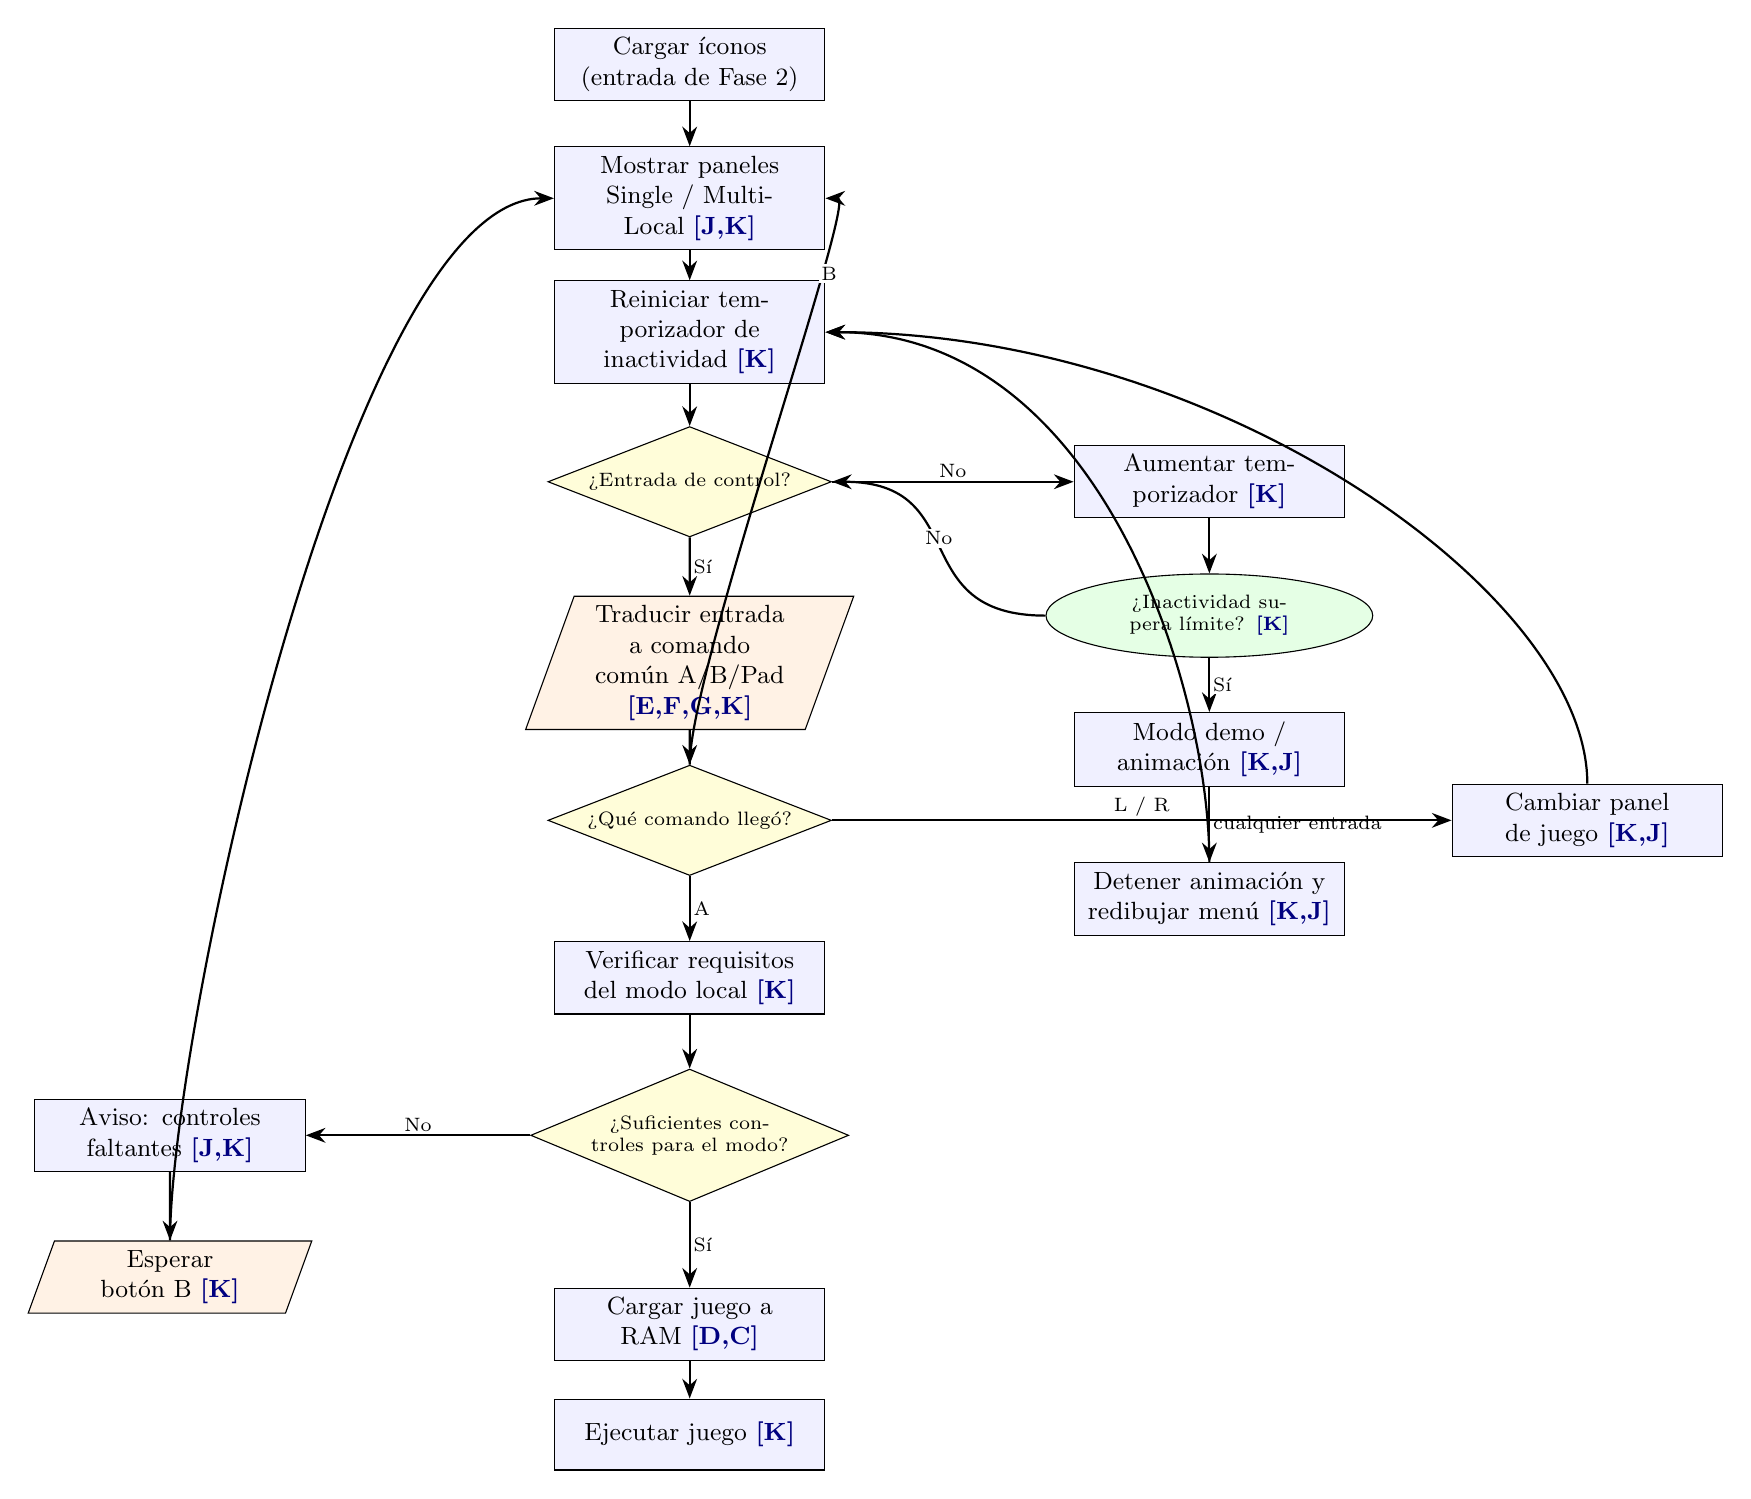
\begin{tikzpicture}[node distance=0.65cm]
% --- columna central (tronco principal) ---
\node (loadicons2) [process] at (0,0) {Cargar \'iconos (entrada de Fase 2)};
\node (showmenu) [process] at (0,-1.7) {Mostrar paneles Single / Multi-Local \grp{J,K}};
\node (resettimer) [process] at (0,-3.4) {Reiniciar temporizador de inactividad \grp{K}};
\node (idle) [decision] at (0,-5.3) {\textquestiondown Entrada de control?};
\node (translate) [io] at (0,-7.6) {Traducir entrada a comando com\'un A/B/Pad \grp{E,F,G,K}};
\node (nav) [decision] at (0,-9.6) {\textquestiondown Qu\'e comando lleg\'o?};
\node (validate) [process] at (0,-11.6) {Verificar requisitos del modo local \grp{K}};
\node (multichk) [decision] at (0,-13.6) {\textquestiondown Suficientes controles para el modo?};
\node (loadgame) [process] at (0,-16.0) {Cargar juego a RAM \grp{D,C}};
\node (rungame) [process] at (0,-17.4) {Ejecutar juego \grp{K}};

% --- columna derecha A (screensaver / inactividad) ---
\node (tick) [process] at (6.6,-5.3) {Aumentar temporizador \grp{K}};
\node (timerchk) [check] at (6.6,-7.0) {\textquestiondown Inactividad supera l\'imite? \grp{K}};
\node (demo) [process] at (6.6,-8.7) {Modo demo / animaci\'on \grp{K,J}};
\node (exitdemo) [process] at (6.6,-10.6) {Detener animaci\'on y redibujar men\'u \grp{K,J}};

% --- columna derecha B (cambio de panel) ---
\node (switchpanel) [process] at (11.4,-9.6) {Cambiar panel de juego \grp{K,J}};

% --- columna izquierda (faltan controles) ---
\node (errprompt) [process] at (-6.6,-13.6) {Aviso: controles faltantes \grp{J,K}};
\node (waitb) [io] at (-6.6,-15.4) {Esperar bot\'on B \grp{K}};

% --- flechas tronco principal ---
\draw[arrow] (loadicons2) -- (showmenu);
\draw[arrow] (showmenu) -- (resettimer);
\draw[arrow] (resettimer) -- (idle);
\draw[arrow] (idle) -- node[lbl,right]{S\'i} (translate);
\draw[arrow] (translate) -- (nav);
\draw[arrow] (nav) -- node[lbl,right]{A} (validate);
\draw[arrow] (validate) -- (multichk);
\draw[arrow] (multichk) -- node[lbl,right]{S\'i} (loadgame);
\draw[arrow] (loadgame) -- (rungame);

% --- ramal de inactividad ---
\draw[arrow] (idle.east) -- node[lbl,above]{No} (tick.west);
\draw[arrow] (tick) -- (timerchk);
\draw[arrow] (timerchk) -- node[lbl,right]{S\'i} (demo);
\draw[arrow] (timerchk.west) .. controls +(left:1.8cm) and +(right:1.8cm) .. node[lbl,pos=0.5,above]{No} (idle.east);
\draw[arrow] (demo) -- node[lbl,right]{cualquier entrada} (exitdemo);
\draw[arrow] (exitdemo.north) .. controls +(up:2.2cm) and +(right:3.5cm) .. (resettimer.east);

% --- ramal L/R (cambiar panel) ---
\draw[arrow] (nav.east) -- node[lbl,above]{L / R} (switchpanel.west);
\draw[arrow] (switchpanel.north) .. controls +(up:2.4cm) and +(right:5cm) .. (resettimer.east);

% --- B vuelve al menu ---
\draw[arrow] (nav.north) .. controls +(up:1.2cm) and +(right:0.4cm) .. node[lbl,pos=0.75,right]{B} (showmenu.east);

% --- ramal de controles faltantes ---
\draw[arrow] (multichk.west) -- node[lbl,above]{No} (errprompt.east);
\draw[arrow] (errprompt) -- (waitb);
\draw[arrow] (waitb.north) .. controls +(up:2.6cm) and +(left:2.6cm) .. (showmenu.west);
\end{tikzpicture}}
\end{center}

\subsection{Descripci\'on}
Esta fase implementa un men\'u con \emph{screensaver} por inactividad
(temporizador reiniciado ante cualquier entrada; al superar el umbral se
entra en modo demo, del cual se sale con cualquier entrada nueva) y la
navegaci\'on est\'andar de una consola: \texttt{L/R} cambia de panel,
\texttt{A} valida e intenta cargar el modo seleccionado, \texttt{B} regresa
al men\'u. La validaci\'on de requisitos (\texttt{MultiCheck}) evita cargar
un modo que necesite m\'as controles de los detectados en la Fase 2.

\begin{algorithm}[H]
\caption{Fase 3 --- Navegaci\'on y selecci\'on local}
\begin{algorithmic}[1]
\State mostrar\_menu(); timer\_idle $\gets 0$
\Loop
    \If{hay\_entrada\_de\_control()}
        \State timer\_idle $\gets 0$
        \State cmd $\gets$ traducir\_a\_comando\_comun()
        \If{cmd = L \textbf{or} cmd = R}
            \State cambiar\_panel(); \textbf{continue}
        \ElsIf{cmd = A}
            \If{suficientes\_controles(modo\_actual)}
                \State cargar\_juego\_a\_ram(); ejecutar\_juego() \Comment{Fase 4}
            \Else
                \State avisar\_controles\_faltantes(); esperar\_boton\_B(); mostrar\_menu()
            \EndIf
        \ElsIf{cmd = B}
            \State mostrar\_menu()
        \EndIf
    \Else
        \State timer\_idle $\gets$ timer\_idle $+ 1$
        \If{timer\_idle $>$ l\'imite}
            \State modo\_demo() \Comment{hasta nueva entrada}
        \EndIf
    \EndIf
\EndLoop
\end{algorithmic}
\end{algorithm}

% =============================================================
\section{Fase 4 --- Ejecuci\'on, audio y seguridad en caliente}
\label{sec:fase4}

\subsection{Diagrama}
\begin{center}
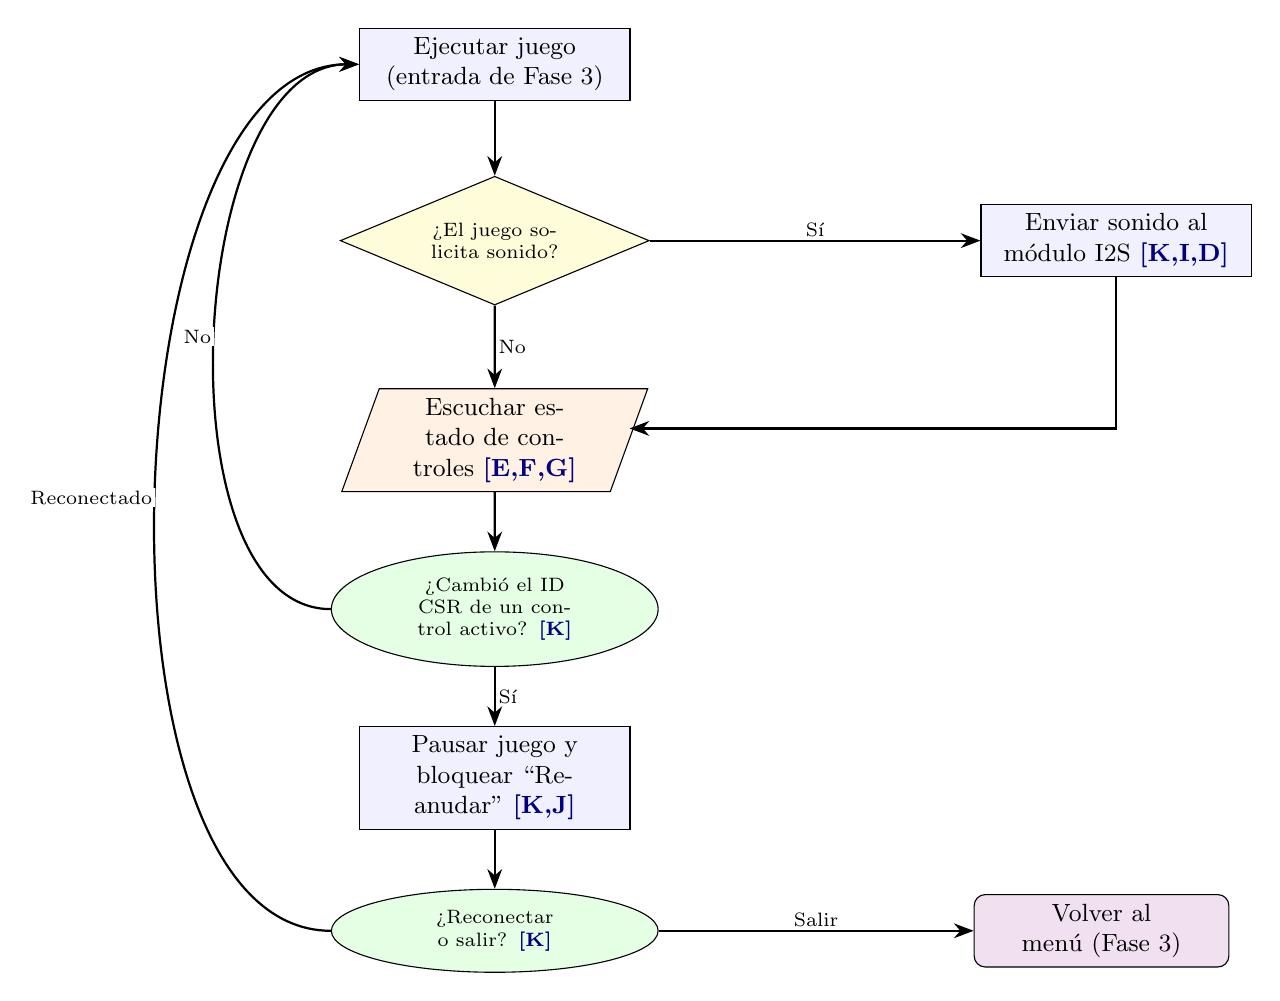
\begin{tikzpicture}[node distance=0.75cm and 2.2cm]
\node (rungame2) [process] {Ejecutar juego (entrada de Fase 3)};
\node (soundchk) [decision, below=of rungame2, yshift=-0.2cm] {\textquestiondown El juego solicita sonido?};
\node (playsound) [process, right=of soundchk, xshift=2.0cm] {Enviar sonido al m\'odulo I2S \grp{K,I,D}};
\node (monitoring) [io, below=of soundchk, yshift=-0.3cm] {Escuchar estado de controles \grp{E,F,G}};
\node (hotplug) [check, below=of monitoring] {\textquestiondown Cambi\'o el ID CSR de un control activo? \grp{K}};
\node (pause) [process, below=of hotplug] {Pausar juego y bloquear ``Reanudar'' \grp{K,J}};
\node (reconnect) [check, below=of pause] {\textquestiondown Reconectar o salir? \grp{K}};

\draw[arrow] (rungame2) -- (soundchk);
\draw[arrow] (soundchk) -- node[lbl,above]{S\'i} (playsound);
\draw[arrow] (playsound.south) |- ($(monitoring.east)+(0,0.15)$);
\draw[arrow] (soundchk) -- node[lbl,right]{No} (monitoring);
\draw[arrow] (monitoring) -- (hotplug);
\draw[arrow] (hotplug) -- node[lbl,right]{S\'i} (pause);
\draw[arrow] (hotplug.west) .. controls +(left:2.2cm) and +(left:2.2cm) .. node[lbl,pos=0.5,left]{No} (rungame2.west);
\draw[arrow] (pause) -- (reconnect);
\draw[arrow] (reconnect.west) .. controls +(left:3.2cm) and +(left:3.2cm) .. node[lbl,pos=0.5,left]{Reconectado} (rungame2.west);
\node (showmenu2) [startstop, right=of reconnect, xshift=1.8cm] {Volver al men\'u (Fase 3)};
\draw[arrow] (reconnect) -- node[lbl,above]{Salir} (showmenu2);
\end{tikzpicture}
\end{center}

\subsection{Descripci\'on}
Durante la ejecuci\'on, el firmware atiende solicitudes de audio del juego
(enviadas al m\'odulo I2S) y, en cada iteraci\'on, vigila el registro CSR de
identificaci\'on de los perif\'ericos activos. Si el \texttt{ID} de un control
que estaba en uso cambia --lo cual indica una desconexi\'on o intercambio en
caliente-- el juego se pausa y se bloquea la opci\'on de reanudar hasta que el
mismo tipo de control vuelva a conectarse o el usuario decida salir al men\'u.
Este mecanismo depende directamente de que el mapa de memoria exponga un
registro de identificaci\'on est\'atico y legible por polling en cada
perif\'erico de entrada (Grupos E, F, G).

\begin{algorithm}[H]
\caption{Fase 4 --- Ejecuci\'on, audio y hot-plugging}
\begin{algorithmic}[1]
\While{jugando}
    \If{juego\_solicita\_sonido()} enviar\_a\_i2s() \EndIf
    \State escuchar\_estado\_controles()
    \If{id\_csr\_cambio(control\_activo)}
        \State pausar\_juego(); bloquear\_reanudar()
        \Repeat
            \State esperar\_evento()
        \Until{reconectado \textbf{or} usuario\_pide\_salir}
        \If{usuario\_pide\_salir}
            \State \textbf{volver a Fase 3 (mostrar\_menu)}
        \EndIf
    \EndIf
\EndWhile
\end{algorithmic}
\end{algorithm}

% =============================================================
\section{Puntos pendientes y observaciones de revisi\'on}
\label{sec:pendientes}

El flujo es l\'ogicamente completo y coherente con la arquitectura de bus CSR
del SoC (ning\'un nodo queda sin salida, todos los ciclos cierran correctamente
y los dos niveles de fallo --duro y blando-- est\'an bien diferenciados). Se
dejan documentados, sin embargo, los siguientes puntos abiertos detectados en
la revisi\'on, que deben resolverse antes de pasar a la etapa de RTL/ASM:

\begin{enumerate}[leftmargin=1.4em]
    \item \textbf{Detecci\'on del control NES (Grupo G).} A diferencia de
    PS/2, el protocolo NES no expone un comando de identificaci\'on est\'andar.
    Debe definirse expl\'icitamente en la especificaci\'on de \texttt{perip\_nes.v}
    si la detecci\'on se resuelve mediante (a)~un adaptador que emula una
    firma PS/2 falsa, o (b)~un pin dedicado de presencia f\'isica, con
    confirmaci\'on manual desde el men\'u.
    \item \textbf{Correspondencia ``2 puertos'' vs. 3 perif\'ericos CSR.} El
    flujo escanea 2 puertos f\'isicos (uno PS/2 combinado + uno NES), mientras
    que el mapa de memoria expone 3 registros CSR independientes (teclado,
    mouse, NES). Debe documentarse expl\'icitamente en la especificaci\'on de
    registros c\'omo el puerto PS/2 f\'isico \'unico se traduce a los dos
    rangos CSR de teclado y mouse.
    \item \textbf{Umbral del temporizador de inactividad.} El flowchart no
    fija un valor num\'erico; debe incorporarse a la tabla de constantes del
    firmware (\texttt{software\_juegos}, Grupo K).
    \item \textbf{M\'odulos con subdiagrama a\'un no desarrollado.} Las
    p\'aginas de flujo espec\'ificas para \texttt{I2S}, \texttt{F-Mouse} y
    \texttt{Flash} dentro del archivo fuente est\'an a nivel de esbozo y deben
    completarse por los equipos responsables antes del checkpoint de RTL
    simulado.
    \item \textbf{Interacci\'on I2C / EEPROM (Grupo H).} No forma parte del
    flujo principal aqu\'i documentado (arranque--men\'u--ejecuci\'on); se
    dispara as\'incronamente al finalizar una partida (guardado de puntajes)
    y debe especificarse en un documento de flujo independiente, ya
    esbozado en las p\'aginas ``H.1'' y ``H.2'' del archivo original.
\end{enumerate}

\end{document}
